\documentclass[11pt]{article}
\usepackage[margin=1in]{geometry}
\usepackage{amsmath,amssymb}
\usepackage{siunitx}
\usepackage{physics}
\usepackage{tikz}
\usetikzlibrary{arrows.meta,angles,quotes,calc,decorations.pathmorphing,decorations.markings}
\usepackage{enumitem}
\sisetup{per-mode=symbol}

\newcommand{\ans}[1]{\boxed{\displaystyle #1}}

\title{PHYS 121 --- HW2 Solutions}

\begin{document}
\maketitle
\setlist[itemize]{noitemsep,topsep=2pt}

% Helper constants
\def\g{\,\mathrm{g}}

\section*{Q1. Spider-Man Swing (Tension \/ Strength)}
Bottom of arc (radius $L$). Forces: tension $T$ up along string, weight $mg$ down. Centripetal: $T - mg = m v^2/L$. Hence
\[ T = m\,\frac{v^2}{L} + mg. \]
Assume traffic speed $\approx\SI{13}{m/s}$, so $v\approx\SI{26}{m/s}$; take $m=\SI{75}{kg}$, $L\approx\SI{75}{m}$ (25 floors). Then
\[ T \approx 75\cdot\frac{26^2}{75}+75\cdot9.8 \approx \SI{1410}{N}. \]
Minimum silk diameter from allowable stress $\sigma$ (take dragline silk $\sigma\approx\SI{1.0e9}{Pa}$): area $A=T/\sigma$, $d=2\sqrt{A/\pi}$:
\[ A\approx1.41\times10^{-6}\,\mathrm{m^2},\quad \ans{d_{\min}\approx\SI{1.34}{mm}}. \]
For equal safety, the better cord is the one with higher allowable stress (smaller required diameter). Dragline silk (\(\sim\)\SI{1}{GPa}) outperforms typical nylon rope (\(\sim\)\SI{0.08}{--}\SI{0.10}{GPa}).

\begin{center}
\begin{tikzpicture}[scale=0.9]
  \coordinate (O) at (0,0);
  \coordinate (B) at (0,-3);
  \draw[thick] (O) -- (B);
  \fill (B) circle (2pt);
  \draw[-{Latex}] (B) -- ++(0,-1) node[below]{$mg$};
  \draw[-{Latex}] (B) -- (O) node[midway,left]{\small $T$};
  \draw[dashed] (-3,0) arc (180:360:3);
  \node[right] at (1.5,-3.2){bottom of swing};
\end{tikzpicture}
\end{center}

\section*{Q2. Motorboat Terminal Speed}
Given $m=\SI{190}{kg}$, thrust $F_T=\SI{40.0}{N}$, linear drag $b\,v$ with $b=\SI{2}{N\,s/m}$. Newton's 2nd law gives
\[ m\,\frac{dv}{dt}=F_T-bv. \]
\begin{enumerate}[label=(\roman*)]
  \item Rearrange to isolate $v$ and $t$: $\displaystyle \frac{dv}{dt}=\frac{F_T}{m}-\frac{b}{m}v$.
  \item Define the terminal speed $\displaystyle v_\infty=\frac{F_T}{b}$ so that $\frac{dv}{dt}=\frac{b}{m}(v_\infty-v)$.
  \item Separate variables: $\displaystyle \frac{dv}{v_\infty-v}=\frac{b}{m}\,dt$ and integrate from $0$ to $t$ (start from rest):
  \[ -\ln\!\Bigl(1-\frac{v}{v_\infty}\Bigr)=\frac{b}{m}\,t. \]
  \item Solve for $v(t)$: $\displaystyle v(t)=v_\infty\Bigl(1-e^{-(b/m)\,t}\Bigr)$.
\end{enumerate}
Numerics: $\displaystyle v_\infty=\frac{40.0}{2}=\ans{\SI{20}{m/s}}$, and $\displaystyle \frac{b}{m}=\frac{2}{190}=\frac{1}{95}$. The time when $v=0.63\,v_\infty$ is $t\approx\ans{\SI{95}{s}}$ (since $e^{-1}=0.37$).
\smallskip
Checks: (1) As $t\to\infty$, $e^{-(b/m)t}\to0$, so $v\to v_\infty$. (2) At $t\to0$, $\displaystyle \dv{v}{t}=\frac{b}{m}v_\infty=\frac{F_T}{m}$, equal to $F_{\text{net}}/m$ initially (drag $=0$ at rest). Initial acceleration $=\ans{\SI{0.211}{m/s^2}}$.

\begin{center}
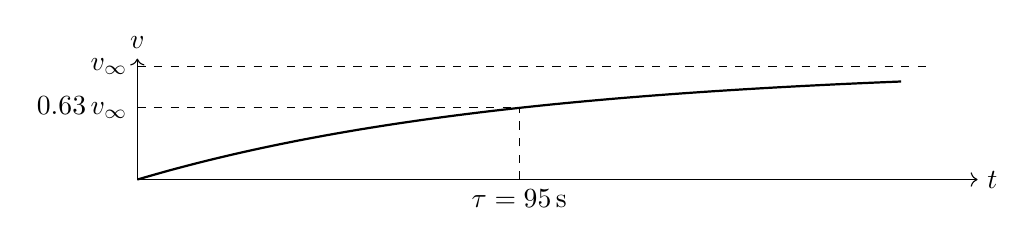
\begin{tikzpicture}[x=0.08\textwidth,y=0.12cm]
  \draw[->] (0,0) -- (11,0) node[right]{$t$};
  \draw[->] (0,0) -- (0,12.8) node[above]{$v$};
  % Curve (scaled so the horizontal asymptote is at y=12 = v_\infty)
  \draw[domain=0:10,smooth,variable=\x,thick] plot (\x,{12*(1-exp(-\x/5))});
  % Mark tau and 0.63 v_\infty
  \draw[dashed] (5,0) -- (5,{12*(1-exp(-1))});
  \node[below] at (5,0){$\tau=\SI{95}{s}$};
  \draw[dashed] (0,{12*(1-exp(-1))}) -- (5,{12*(1-exp(-1))});
  \node[left] at (0,{12*(1-exp(-1))}) {$0.63\,v_\infty$};
  % Mark v_\infty
  \draw[dashed] (0,12) -- (10.4,12);
  \node[left] at (0,12) {$v_\infty$};
\end{tikzpicture}
\end{center}

\section*{Q3. Box up an Incline (constant speed)}
Incline $30^{\circ}$, $m=\SI{45}{kg}$, $\mu_k=0.35$, horizontal $F$. Along the plane (up positive):
\[ F\cos30^{\circ} = mg\sin30^{\circ}+\mu_k\bigl(mg\cos30^{\circ}+F\sin30^{\circ}\bigr). \]
Solve: $\displaystyle F=\frac{mg(\sin30^{\circ}+\mu_k\cos30^{\circ})}{\cos30^{\circ}-\mu_k\sin30^{\circ}}=\ans{\SI{5.13e2}{N}}.$
Distance $s=\SI{8.0}{m}$. Work:
\[ W_F = Fs\cos30^{\circ}=\ans{\SI{3.55e3}{J}},\quad N=mg\cos30^{\circ}+F\sin30^{\circ}\Rightarrow f_k=\mu_k N\approx\SI{224}{N},\]
\[ W_{\!f}=-f_k s=\ans{\SI{-1.79e3}{J}},\quad W_g=-mg(s\sin30^{\circ})=\ans{\SI{-1.76e3}{J}}. \]
\textit{Signs:} $W_F>0$ because $\vec F$ has a component along the displacement up the plane; $W_{\!f}<0$ since kinetic friction opposes motion; $W_g<0$ since gravity’s component is down the plane while displacement is up the plane; $W_N=0$ because $\vec N\perp$ displacement.
\textit{Check (Work--Energy):} $W_{\text{net}}=\Delta K$. Constant speed $\Rightarrow \Delta K=0\Rightarrow W_{\text{net}}=0$, which our totals satisfy.
Thus $W_{\text{net}}\approx0$ consistent with constant speed.

\begin{center}
\begin{minipage}{0.48\textwidth}\centering
% View 1: World axes (x, y) shown explicitly
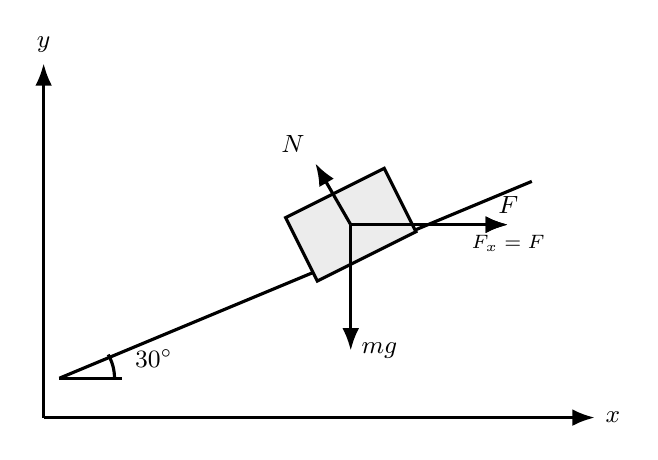
\begin{tikzpicture}[scale=1, line width=0.40mm]
  % Axes
  \draw[-{Latex}] (-3.2,-2.0) -- ++(7.0,0) node[right]{\small $x$};
  \draw[-{Latex}] (-3.2,-2.0) -- ++(0,4.5) node[above]{\small $y$};
  % Incline and block
  \draw (-3,-1.5) -- (3,1);
  % Block centered at C, aligned with incline (~26.565°)
  % Block reference point (center)
  \coordinate (C) at (0.7,0.45);
  \begin{scope}[shift={(C)}, rotate=26.565]
    \draw[fill=gray!15] (-0.7,-0.45) rectangle (0.7,0.45);
  \end{scope}
  % Forces
  \draw[-{Latex}] (C) -- ++(2,0) node[above]{\small $F$};
  \draw[-{Latex}] (C) -- ++(0,-1.6) node[right]{\small $mg$};
  \draw[-{Latex}] (C) -- ++(-0.45,0.78) node[above left]{\small $N$};
  % Components of F in world axes: F_x = F, F_y = 0
  \draw[dashed,-{Latex}] (C) -- ++(2,0) node[below]{\scriptsize $F_x=F$};
  % Angle marker 30° at left contact point of incline
  \draw (-3,-1.5) -- ++(0.8,0);
  \draw (-2.3,-1.5) ++(0,0) arc (0:30:0.6);
  \node at (-1.8,-1.25) {\small $30^{\circ}$};
\end{tikzpicture}
\end{minipage}\hfill
\begin{minipage}{0.48\textwidth}\centering
% View 2: Axes aligned with incline (s along plane, n normal)
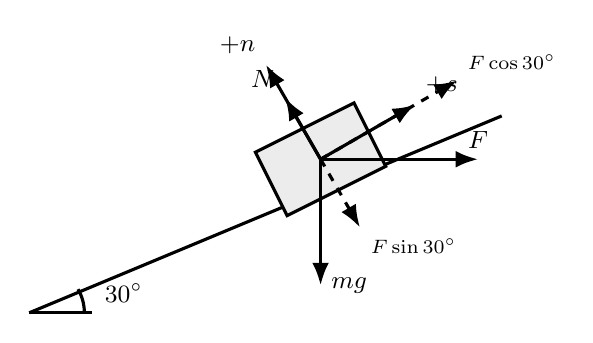
\begin{tikzpicture}[scale=1, line width=0.40mm]
  % Incline and block
  \draw (-3,-1.5) -- (3,1);
  % Block centered at C, aligned with incline (~26.565°)
  % Block reference point (center)
  \coordinate (C) at (0.7,0.45);
  \begin{scope}[shift={(C)}, rotate=26.565]
    \draw[fill=gray!15] (-0.7,-0.45) rectangle (0.7,0.45);
  \end{scope}
  % s-n axes at the block
  \draw[-{Latex}] (C) -- ++(1.2,0.6928) node[above right]{\small $+s$};
  \draw[-{Latex}] (C) -- ++(-0.6928,1.2) node[above left]{\small $+n$};
  % Forces
  \draw[-{Latex}] (C) -- ++(2,0) node[above]{\small $F$};
  \draw[-{Latex}] (C) -- ++(0,-1.6) node[right]{\small $mg$};
  \draw[-{Latex}] (C) -- ++(-0.45,0.78) node[above left]{\small $N$};
  % Components of F along +s and -n
  \draw[dashed,-{Latex}] (C) -- ++({2*cos(30)},{2*sin(30)}) node[above right]{\scriptsize $F\cos30^{\circ}$};
  \draw[dashed,-{Latex}] (C) -- ++({sin(30)},{-cos(30)}) node[below right]{\scriptsize $F\sin30^{\circ}$};
  % Angle marker 30° at left contact point of incline
  \draw (-3,-1.5) -- ++(0.8,0);
  \draw (-2.3,-1.5) ++(0,0) arc (0:30:0.6);
  \node at (-1.8,-1.25) {\small $30^{\circ}$};
\end{tikzpicture}
\end{minipage}
\end{center}
\smallskip
{\small\emph{Incline-aligned view is better for writing component equations; world-axes view is good for visualization.}}

\section*{Q4. Vertical Spring Gun}
$k=\SI{14}{N/cm}=\SI{1400}{N/m}$, $m=\SI{15}{g}$, top is \SI{5.0}{m} above the uncompressed end. Energy from compressed to top (include rise by $x$ while leaving):
\[ \tfrac12 kx^2 = mg(5.0 + x). \]
Quadratic $700x^2-0.147x-0.735=0$ gives physical root $\ans{x\approx\SI{3.25}{cm}}$.

\begin{center}
\begin{tikzpicture}[scale=1]
  \draw[thick] (0,0) -- (0,2);
  \draw[decorate,decoration={zigzag,segment length=5,amplitude=2}] (0,0) -- (0,1.2);
  \fill (0,1.2) circle (2pt);
  \draw[<->] (0.2,1.2) -- node[right]{\small $x$} (0.2,2);
  \draw[<->] (-0.5,2) -- node[left]{\small 5.0 m} (-0.5,6.2);
\end{tikzpicture}
\end{center}

\section*{Q5. Kinetic Energy of a Massive Spring}

\textbf{Rod model:} Consider a rod of length $L$ and total mass $M$. At position $x$ (measured from one end, $0\le x\le L$), take a slice of length $dx$. The mass of this slice is $dm=(M/L)dx$, where $M/L$ is the linear mass density. If the rod has a linear speed profile $v(x)=(x/L)v$ (where $v$ is the speed at the far end $x=L$), then each slice moves with speed $v(x)$.

\begin{center}
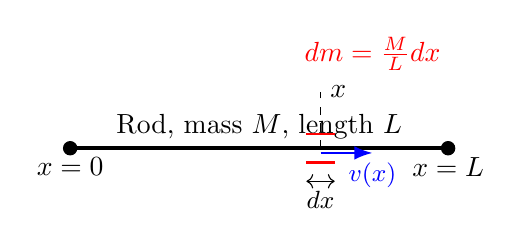
\begin{tikzpicture}[scale=1.2]
  % Rod
  \draw[ultra thick] (0,0) -- (4,0);
  % Mark endpoints
  \draw[fill=black] (0,0) circle (2pt) node[below]{$x=0$};
  \draw[fill=black] (4,0) circle (2pt) node[below]{$x=L$};
  % Label rod
  \node[above] at (2,0) {Rod, mass $M$, length $L$};
  % Draw a slice at position x
  \draw[thick,red] (2.5,0.15) -- (2.8,0.15);
  \draw[thick,red] (2.5,-0.15) -- (2.8,-0.15);
  \draw[<->] (2.5,-0.35) -- (2.8,-0.35) node[midway,below]{\small $dx$};
  \draw[dashed] (2.65,0) -- (2.65,0.6);
  \node[right] at (2.65,0.6) {$x$};
  % Velocity vector
  \draw[-{Latex},blue,thick] (2.65,-0.05) -- (3.2,-0.05) node[right,below]{\small $v(x)$};
  % Mass label
  \node[red] at (3.2,1) {$dm=\frac{M}{L}dx$};
\end{tikzpicture}
\end{center}

\textbf{Kinetic energy element:} The kinetic energy of the slice at position $x$ is
\[ dK = \tfrac12 dm\,v(x)^2 = \tfrac12 \frac{M}{L}\left(\frac{x}{L}v\right)^2dx = \tfrac12 \frac{M v^2}{L^3} x^2\,dx. \]

\textbf{Integration:} The total kinetic energy is obtained by integrating $dK$ from $x=0$ to $x=L$:
\[ K = \int_0^L dK = \frac{M v^2}{2L^3}\int_0^L x^2\,dx = \frac{M v^2}{2L^3}\cdot\frac{L^3}{3} = \ans{\tfrac16 M v^2}. \]

\textbf{Comparison with point-mass result:} For a point mass of mass $M$ moving at speed $v$, the kinetic energy would be $K_{\text{point}} = \tfrac12 M v^2$. Our result is $\tfrac16 M v^2$, which is exactly \textit{one-third} of the point-mass result.

\textbf{Explanation:} The difference arises because the rod has a \textit{distribution of speeds}. In our model, only the far end ($x=L$) moves at speed $v$; parts closer to $x=0$ move slower (e.g., the center at $x=L/2$ moves at $v/2$). Since kinetic energy depends on $v^2$, the slower-moving parts contribute less energy than if the entire mass were moving at speed $v$. The factor of $1/3$ reflects the quadratic averaging over the linear speed profile: $\langle v^2 \rangle = \frac{1}{L}\int_0^L \left(\frac{x}{L}v\right)^2 dx = \frac{v^2}{3}$.

\section*{Q6. Power, Drag, and Fuel}
At $v=\SI{15}{m/s}$, power to wheels $P_{15}=\SI{20}{hp}=\SI{1.492e4}{W}$. (i) Constant drag $F_d$:
\[ F_d=\frac{P_{15}}{v}=\ans{\SI{9.95e2}{N}},\quad P_{30}=F_d\,(\SI{30}{m/s})=\ans{\SI{2.98e4}{W}}\ (\approx\SI{40}{hp}). \]
Energy for \SI{10}{km}: $W=F_d d=\ans{\SI{9.95e6}{J}}$ to wheels; fuel energy (25\% efficiency): $\ans{\SI{3.98e7}{J}}$ at either speed.

(ii) Linear drag $F_d=kv$ matched at \SI{15}{m/s}: $k=F_d/v=\ans{\SI{66.3}{N\,s/m}}$. Then
\[ P(v)=kv^2,\ P_{30}=k(30)^2=\ans{\SI{5.97e4}{W}}\ (\approx\SI{80}{hp}). \]
Energy for \SI{10}{km}: $W=kv d$ gives $W_{15}=\ans{\SI{9.95e6}{J}}$, $W_{30}=\ans{\SI{1.99e7}{J}}$; fuel energies are 4\,$\times$ these.

\textbf{Reflection:} In (i) doubling speed doubles power and leaves energy per distance unchanged; in (ii) doubling speed quadruples power and doubles energy per distance. Real driving matches the trend that higher speed needs much more power and fuel per mile. Aerodynamic drag is approximately quadratic, $F\propto v^2$, so realistically $P\propto v^3$ and energy per distance $\propto v^2$, which increases even faster with speed than our linear-drag model predicts.

\section*{Q7. Peg and Complete Loop}
Release from horizontal, length $a$. After catching the peg, the small-circle radius is $a-h$.

\begin{itemize}
  \item Energy (release $\to$ bottom of big circle, drop $a$):
  \[ mg\,a = \tfrac12 m v_b^2 \quad\Rightarrow\quad v_b^2 = 2ga,\quad v_b=\sqrt{2ga}. \]
  \item Energy (bottom $\to$ top of small circle, rise $2(a-h)$):
  \[ \tfrac12 m v_b^2 = \tfrac12 m v_t^2 + mg\,2(a-h)
     \quad\Rightarrow\quad v_t^2 = v_b^2 - 4g(a-h) = 2ga - 4g(a-h),\quad v_t=\sqrt{2ga-4g(a-h)}. \]
\end{itemize}

Non-slack at the top requires a strictly positive tension. At the top, taking inward as positive, the radial balance is
\[ T + mg = m\,\frac{v_t^2}{a-h} \quad\Rightarrow\quad T = m\,\frac{v_t^2}{a-h} - mg. \]
Requiring $T>0$ gives
\[ v_t^2 > g\,(a-h). \]
Using $v_t^2 = 2ga - 4g(a-h)$ gives $2a - 4(a-h) > (a-h)$, i.e., $-2a + 4h > a - h$.
Hence $5h > 3a$, so \ans{h > \tfrac{3}{5}a}.

\section*{Q8. Bungee Jump Estimate}
Mass $\SI{72}{kg}$, free fall \SI{15}{m} before stretch; spring $k=\SI{50}{N/m}$. Energy from platform to lowest point:
\[ mg(15+x)=\tfrac12 k x^2. \]
Solve $25x^2-705.6x-10584=0$ for $x>0$: $\ans{x\approx\SI{39.1}{m}}$. Total drop $\ans{15+x\approx\SI{54.1}{m}}$.

\begin{center}
\begin{minipage}{0.45\textwidth}\centering
\textbf{Free fall (no stretch)}
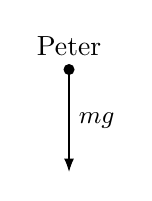
\begin{tikzpicture}[scale=1]
  \fill (0,0) circle (2pt);
  \draw[-{Latex}] (0,0) -- (0,-1.3) node[midway,right]{\small $mg$};
  \node[above] at (0,0.05) {Peter};
\end{tikzpicture}
\end{minipage}\hfill
\begin{minipage}{0.45\textwidth}\centering
\textbf{During stretch}
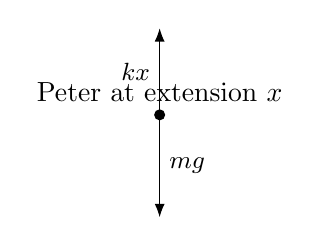
\begin{tikzpicture}[scale=1]
  \fill (0,0) circle (2pt);
  \draw[-{Latex}] (0,0) -- (0,-1.3) node[midway,right]{\small $mg$};
  \draw[-{Latex}] (0,0) -- (0,1.1) node[midway,left]{\small $k x$};
  \node[above] at (0,0.05) {Peter at extension $x$};
\end{tikzpicture}
\end{minipage}
\end{center}

\section*{Q9. Bullet + Block (inelastic)}
$m_b=\SI{0.220}{kg}$ at $v_i=\SI{400}{m/s}$ embeds into $M=\SI{1.30}{kg}$ on a frictionless table. Momentum conservation:
\[ v_f=\frac{m_b v_i}{m_b+M}=\ans{\SI{57.9}{m/s}}\ (\text{east}). \]
Impulses: $J_b = m_b(v_f-v_i)=\ans{\SI{-75.3}{N\,s}}$ (on bullet, west), $J_M = M v_f=\ans{\SI{75.3}{N\,s}}$ (on block, east). Over \SI{3}{ms}: $\ans{\overline F\approx\SI{2.51e4}{N}}$.

\begin{center}
\begin{minipage}{0.48\textwidth}\centering
\textbf{Before (east positive)}
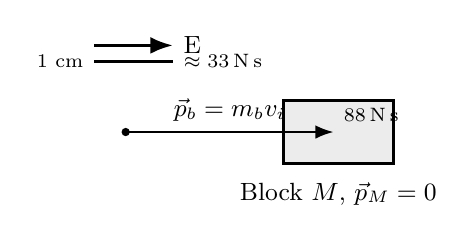
\begin{tikzpicture}[scale=1, line width=0.40mm]
  % Compass and scale bar
  \draw[-{Latex}] (-2.4,1.1) -- (-1.4,1.1) node[right]{\small E};
  \draw (-2.4,0.9) -- (-1.4,0.9);
  \node[left] at (-2.4,0.9) {\scriptsize 1 cm};
  \node[right] at (-1.4,0.9) {\scriptsize $\approx 33\,\mathrm{N\,s}$};
  % Block at rest
  \draw[fill=gray!15] (0,-0.4) rectangle (1.4,0.4);
  \node[below] at (0.7,-0.5){\small Block $M$, $\vec p_M=0$};
  % Bullet approaching from left; momentum vector scaled: 2.64 cm = 88 N s
  \fill (-2,0) circle (1.5pt);
  \draw[-{Latex},thick] (-2,0) -- ++(2.64,0)
    node[midway,above]{\small $\vec p_b = m_b v_i$}
    node[above right]{\scriptsize $88\,\mathrm{N\,s}$};
\end{tikzpicture}
\end{minipage}\hfill
\begin{minipage}{0.48\textwidth}\centering
\textbf{After (perfectly inelastic)}
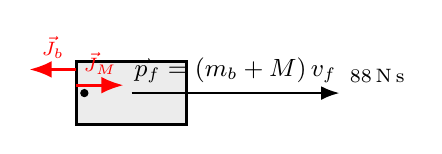
\begin{tikzpicture}[scale=1, line width=0.40mm]
  % Combined block+bullet moving east; momentum vector scaled: 2.64 cm = 88 N s
  \draw[fill=gray!15] (0,-0.4) rectangle (1.4,0.4);
  \fill (0.1,0) circle (1.5pt); % embedded bullet (schematic)
  \draw[-{Latex},thick] (0.7,0) -- ++(2.64,0)
    node[midway,above]{\small $\vec p_f=(m_b+M)\,v_f$}
    node[above right]{\scriptsize $88\,\mathrm{N\,s}$};
  % Impulse pair schematic (equal/opposite)
  \draw[-{Latex},red] (0,0.3) -- (-0.6,0.3) node[midway,above]{\scriptsize $\vec J_b$};
  \draw[-{Latex},red] (0,0.1) -- (0.6,0.1) node[midway,above]{\scriptsize $\vec J_M$};
\end{tikzpicture}
\end{minipage}

\vspace{0.25em}
{\small Vectors drawn to scale: $p_b=p_f=\SI{88}{N\,s}$ east. With $m_b=\SI{0.220}{kg}$, $v_i=\SI{400}{m/s}$, $(m_b+M)v_f=\SI{88}{N\,s}\Rightarrow v_f=\SI{57.9}{m/s}$.}
\end{center}

\noindent\textit{Note: Q10 omitted per course announcement.}

\section*{Bonus. Terminal-speed experiment (0--2 pts)}
\begin{center}
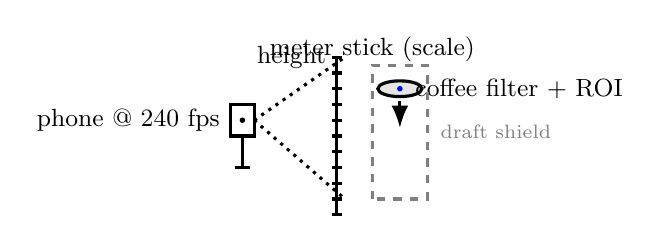
\begin{tikzpicture}[scale=1, line width=0.40mm]
  % Meter stick (2 m span for clarity)
  \draw (0,0) -- (0,2);
  \foreach \y in {0,0.2,...,2} {\draw (-0.06,\y) -- (0.06,\y);} % ticks
  \node[left] at (0,2) {\small height};
  \node at (0.45,2.1) {\small meter stick (scale)};
  % Coffee filter with ROI marker
  \draw[fill=gray!20] (0.8,1.6) ellipse (0.28 and 0.10);
  \fill[blue] (0.8,1.6) circle (1pt);
  \draw[-{Latex}] (0.8,1.45) -- (0.8,1.1);
  \node[right] at (0.86,1.6) {\small coffee filter + ROI};
  % Draft shield (clear bin)
  \draw[gray,dashed] (0.45,0.2) rectangle (1.15,1.9);
  \node[right,gray] at (1.18,1.05) {\scriptsize draft shield};
  % Phone camera on tripod to the left
  \draw (-1.35,1.0) rectangle (-1.05,1.4);
  \fill (-1.20,1.2) circle (1pt);
  \draw (-1.20,1.0) -- (-1.20,0.6);
  \draw (-1.30,0.6) -- (-1.10,0.6);
  \node[left] at (-1.35,1.2) {\small phone @ 240 fps};
  % Field of view guides
  \draw[dotted] (-1.05,1.2) -- (0.1,0.2);
  \draw[dotted] (-1.05,1.2) -- (0.1,2.0);
\end{tikzpicture}
\end{center}

\begin{itemize}
  \item \textbf{Setup}: Indoors, drop a coffee filter beside a vertical meter stick; phone on tripod \(\ge\)240 fps, optical axis perpendicular, use a clear bin as a draft shield and a colored ROI dot on the filter.
  \item \textbf{Data}: Track \(y(t)\) of the ROI every 2--4 frames across 3--5 drops; repeat with 1--4 stacked filters to vary mass and confirm \(v_t\) scaling.
  \item \textbf{Model/fit}: Quadratic drag gives \(v(t)=v_t\tanh( g t/ v_t )\) and the position model \(y(t)=y_0+\tfrac{v_t^2}{g}\ln\!\cosh( g t/ v_t )\); fit \(y(t)\) directly (less noisy) to extract \(v_t\). Linear-drag cross-check: \(v(t)=v_t(1-e^{-t/\tau})\).
  \item \textbf{Uncertainty}: Systematic (parallax, scale skew, timing) and random (drafts, tilt). Mitigate via long camera distance, careful alignment, averaging trials, and verifying that late-time \(v(t)\) plateaus.
\end{itemize}

\section*{Assitance notes:} LLMs were used as translators and concept explainers. No direct solutions were provided.

\end{document}


